\section{\textsc{Book-Embedding} is \NP-Complete}
\label{section:np-complete}

In this section we
construct a polynomial-time reduction from the \NP-complete problem \probBetween, defined below,
to \probBook, \ie we show that \probBook is \NP-complete. Therefore,
we cannot expect there to be an efficient algorithm for solving the general
book embedding problem.

Checking the book constraints for a pair of edges takes $\OO(1)$~time
and there are $\OO\bigl(\sum_{i} |E_i|^2\bigr)$ pairs to check.
Thus, checking the validity of a guessed book order takes polynomial
time and the book embedding problem must, therefore, be in~\NP.

We now give a polynomial time reduction from the problem \probBetween, which was shown to be \NP-complete by Opatrny~\cite{opatrny:79}, to \probBook and, thereby, show that \probBook itself is \NP-complete.

\newProb{\probBetween}{A finite set $M := \range{n}$ and a set of ordered triples $C \subseteq M^3$.}
{Is there a total ordering $<$ of $M$ such that either $a < b < c$ or $a > b > c$ occurs for all $(a, b, c) \in C$?}

The idea of the reduction is to map each triple to edges on two new pages that form a $C_4$, a cycle on 4~vertices. By
the following lemma, these two pages exactly represent the betweenness constraint.

\begin{figure}[\placement]\centering
    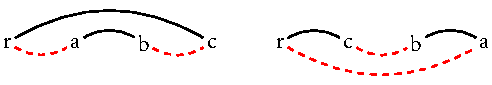
\includegraphics{figures/t_np_c4}
    \caption[Drawings of $C_4$]{The two drawings of a $C_4$ starting at $r$}
    \label{figure:np-c4}
\end{figure}

\begin{lemma}
\label{lemma:np-c4}
Let $V := \{r, a, b, c\}$, $E_1 := \bigl\{\{r, a\},\{b, c\}\bigr\}$ and $E_2 := \bigl\{\{a, b\}, \{r, c\}\bigr\}$. Then
$r < a < b < c$ and $r < c < b < a$, depicted in \myref{figure:np-c4}, are the only valid book embeddings of $E_1$ and $E_2$ with 
$r$ as first vertex.
\end{lemma}
\begin{myproof}
Let $<$ be a valid book order on $V$.
By \myref{lemma:constraints} the two pages yield the constraints $r < b < a \Leftrightarrow r < c < a$
and $r < a < c \Leftrightarrow r < b < c$. Since $r$ is the smallest element of $<$, this
is the same as $b < a \Leftrightarrow c < a \Leftrightarrow c < b$, \ie only the two cases $r < a < b < c$ and
$r < c < b < a$ remain.
\end{myproof}

Now let's do the formal reduction.

\begin{theorem}
\label{lemma:np-hard}
There is a polynomial time reduction from \probBetween to \probBook. Thus,
\probBook is \NP-complete.
\end{theorem}
\begin{myproof}
Let $I := (M, C)$ be a betweenness instance. 

Construct a book embedding instance $f(I) := \bigl(V, \bigcup_{t \in C} \left(E_{t,1} \cup E_{t,2}\right)\bigr)$ as follows.
Take $V := M\,\cup\,\{r\}$ as vertex set where $r \not\in M$ is a new symbol. For each triple $\tau~=~(a, b, c) \in C$ introduce
two new pages $E_{\tau, 1} := \bigl\{\{r, a\}, \{b, c\}\bigr\}$ and $E_{\tau, 2} := \bigl\{\{a, b\},\{r, d\}\bigr\}$. The instance $f(I)$ can obviously 
be computed in polynomial time.

Now show that $I$ is a positive instance if and only $f(I)$ is one.\nopagebreak
\begin{itemize}
\item[``$\Rightarrow$''] Let $I$ be a positive instance of \probBetween with valid total order $<$. Extend~$<$ to $V$ via
$r < k$ for all $k \in M$. For each triple $(a, b, c) \in C$ we have $r < a < b < c$ or $r < c < b < a$, \ie $<$ yields
a valid embedding of the pages by \myref{lemma:np-c4}. Thus, $<$ is a correct solution of $f(I)$.

\item[``$\Leftarrow$''] Let $f(I)$ be a positive instance of \probBook with valid total order~$<$. By \myref{lemma:symmetry} we
can assume  without loss
of generality that~$<$ is rotated such that $r$ is its smallest element. Then we have the situation of \myref{lemma:np-c4} for each triple $\tau = (a, b, c) \in C$ with
the pages~$E_{\tau,1}$ and $E_{\tau,2}$, \ie $a < b < c$ or $c < b < a$. Therefore, the order~$<$ restricted to $M$ is indeed a valid solution of $I$.\qedhere
\end{itemize}
\end{myproof}

We conclude that \probBook is \NP-complete. The reduction of
\myref{lemma:np-hard} gives us even more. The pages it creates are
matchings, \ie even the special case \probNotMatching of book embedding where the
edges on each page form a matching remains \NP-complete.

\newProb{\probNotMatching}{A vertex set $V$ and matchings $E_1, \dotsc, E_k \subseteq \binom{V}{2}$}%
{Is there a book embedding of $(V, E_1), \dotsc, (V, E_k)$?}

We do not know how complex the problem is when the edges on the pages form perfect matchings. This
special case is considered in more detail in \myref{section:matchings}.
%\begin{theorem}
%\label{theorem:np-complete}
%\probBook is \NP-complete.
%\end{theorem}
%\begin{myproof}
%Follows immediately from \myref{lemma:np-hard}.
%\end{myproof}